\chapter{Pug.js}
\label{sec:pug1}
% Old Ch. 5

After an exhausting installation process, let's write some code.
Pug.js (abbreviated as Pug) files are translated into HTML files, they provide the basic structure of the web page. Now let's learn how to write our own web page using Pug.

\section{Logistics}

\subsection*{Where to write my code?}

As discussed in \cref{sec:quickstart}, write the majority of your Pug code inside the \texttt{.container} class in every file under \texttt{templates/views}. 

\begin{lstlisting}[language=pug]
extends ../layouts/default

block content
	.container
		//- Your code goes here...
\end{lstlisting}

The things you write here will be translated into an HTML file matching the name of the file in the \texttt{docs} folder after you have run \texttt{npm run build}. Once again, your should NOT edit anything in the \texttt{docs} folder.

\subsection*{Magic on the Pug.js website}

\textit{This method is not a replacement of your local code. It is useful when you would like to check what is the HTML code generated with the Pug code you supplied, but it cannot let you visualise the elements and see how they would actually look like in the browser.}
\vspace{6mm}

The \href{{https://pugjs.org/}}{Pug.js official website}\footnote{Link: \url{https://pugjs.org/}} contains a detailed documentation on how it is translated to HTML.

What's also valuable is its interactive translator, you can just type any Pug code on any page in the documentation, \href{https://pugjs.org/language/attributes.html}{like this one}\footnote{Link: \url{https://pugjs.org/language/attributes.html}}, type Pug code on the left box and it will translate to HTML code on the right.

\begin{figure}[h]
\centering
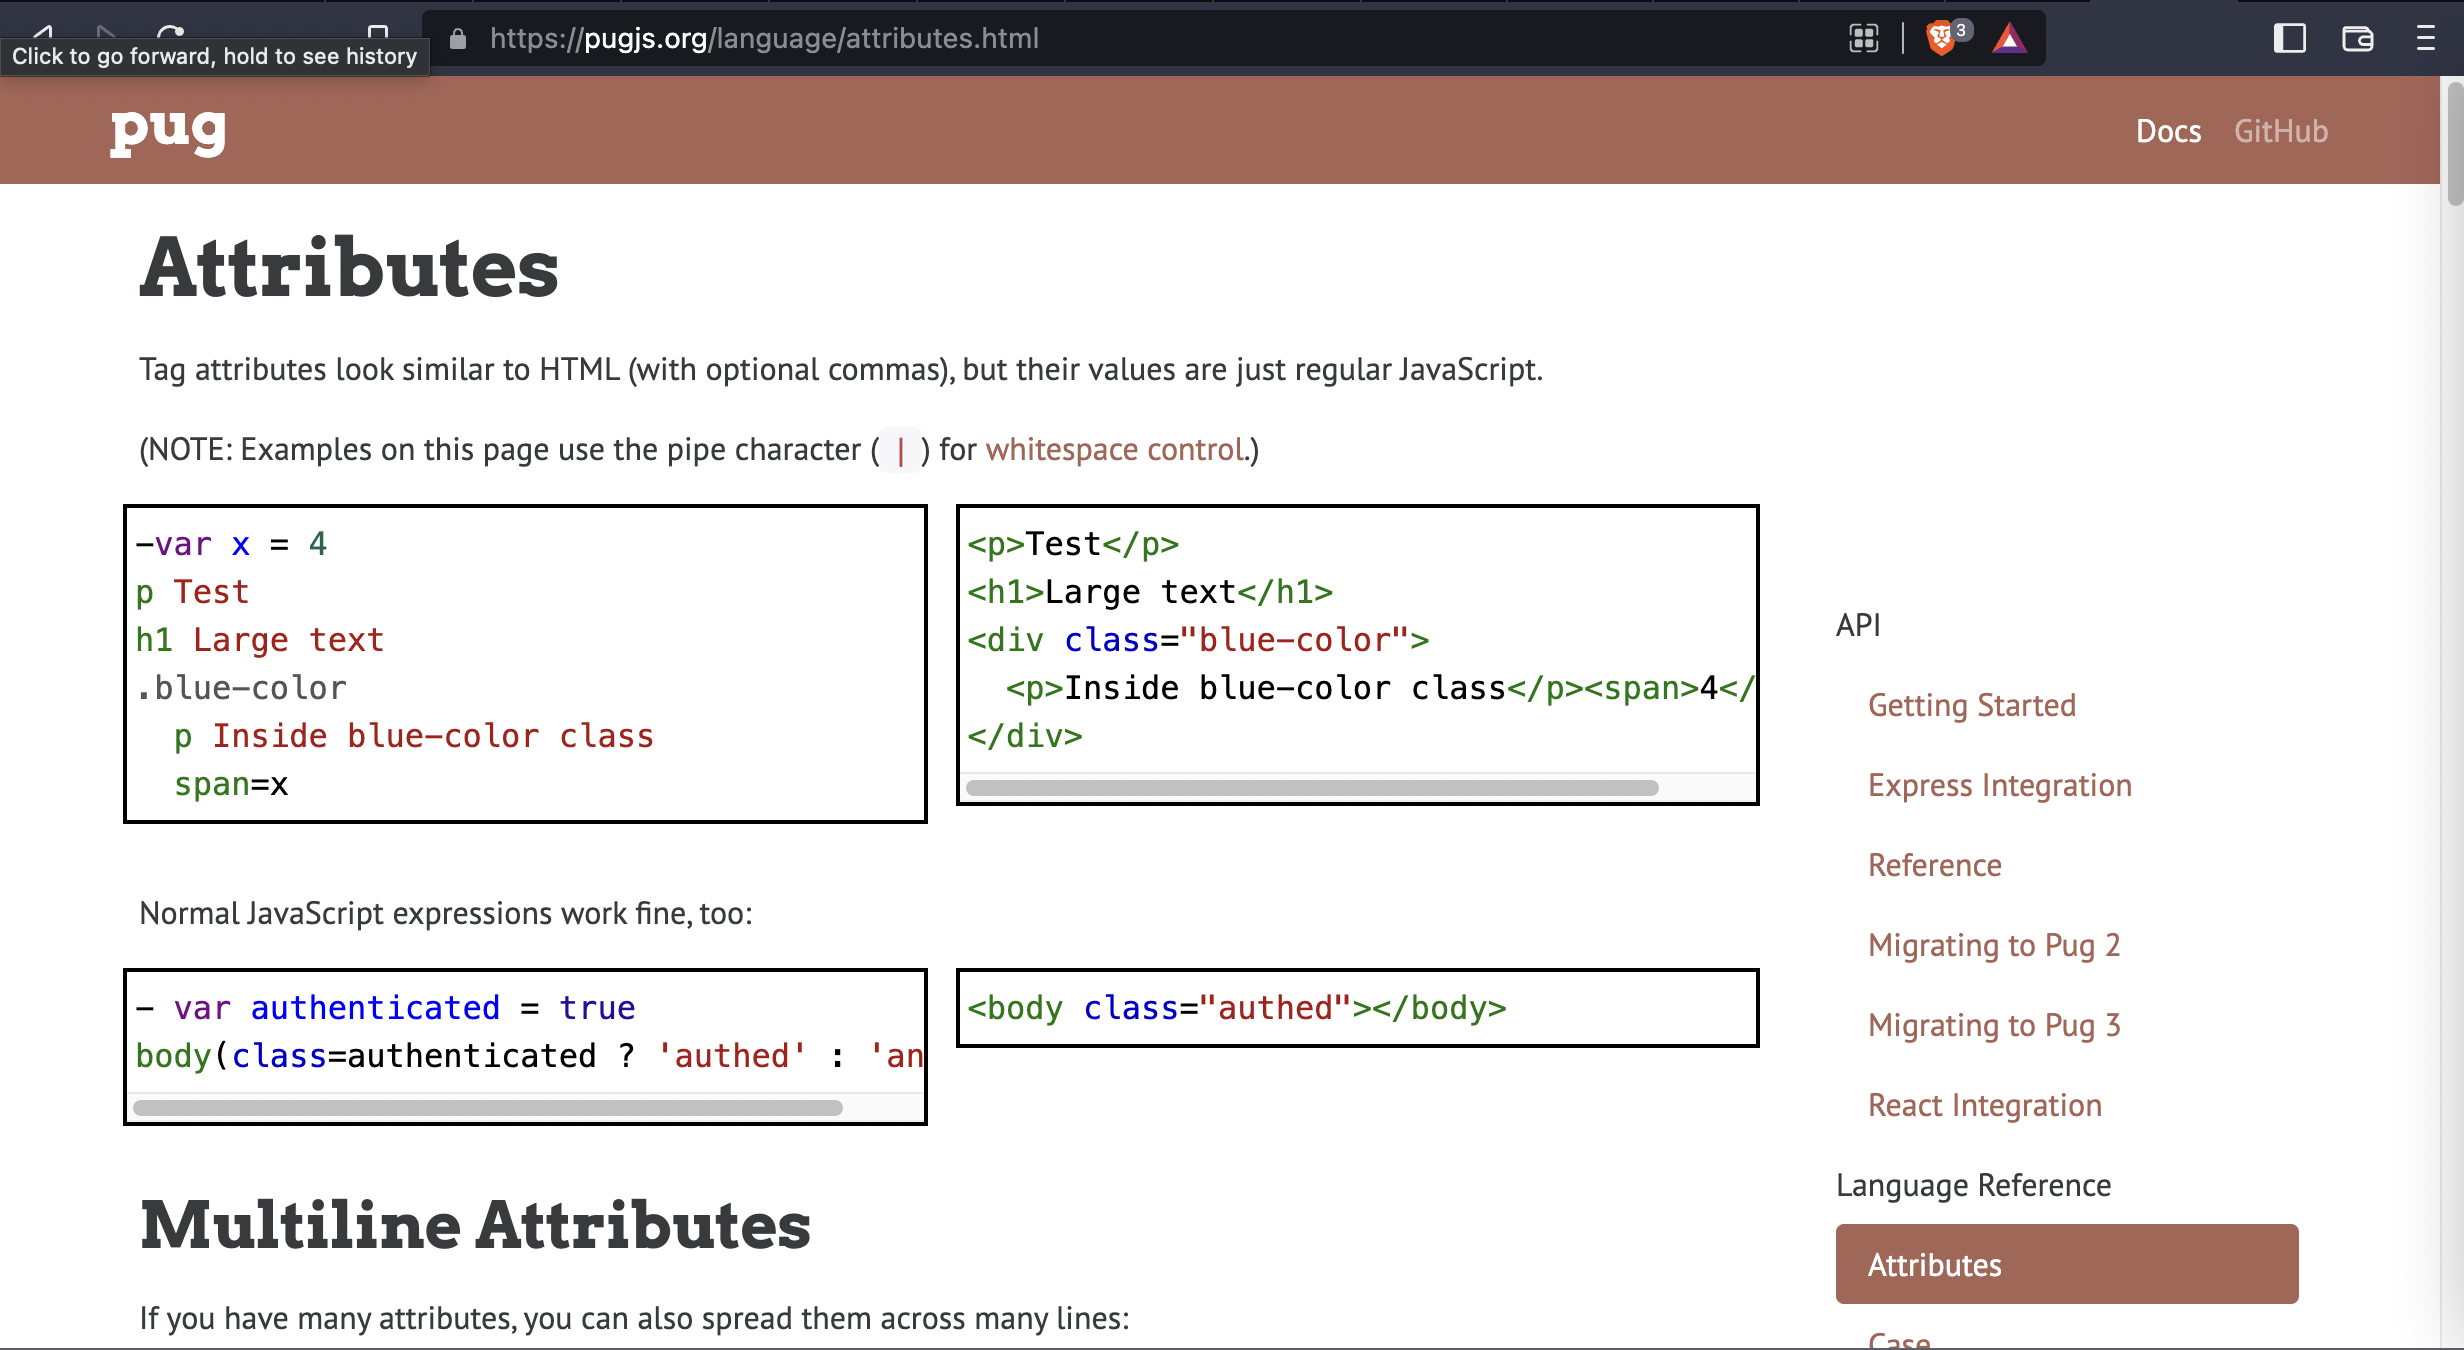
\includegraphics[width=13cm]{images/ch5-puginteractive.png}
\caption{Example usage of the interactive translator on the Pug.js official website}
\end{figure}

\subsection*{Further Resources}

I didn't have this piece of notes back when I first learned Pug. Here is \href{https://youtu.be/kt3cEjjkCZA}{the video}\footnote{Link: \url{https://youtu.be/kt3cEjjkCZA}{the video}} that I used to learn the basics. 

HTML is well documented online. You could refer to the \href{https://www.w3schools.com/tags/default.asp}{w3schools documentation}\footnote{Link: \url{https://www.w3schools.com/tags/default.asp}} to learn how to use some more tags. The common ones are either explained in detail in this piece of notes in this chapter. There is no need to understand all the tags, some are much more useful than the rest. My advice is search online when you don't know how to represent something in HTML, e.g. a table, that's when you know you should learn how to use those tags. The translation to Pug is well described in other parts of this chapter already.

\section{General form of a Pug tag}

Each line of Pug code can be divided into four sections.

\begin{lstlisting}[language=pug]
a#id.class-1.class-2(href="abouts.html") Click for abouts page
\end{lstlisting}

\begin{enumerate}
    \item \textbf{Tag}: Specifies the type of element, can be one of the tags in \cref{fig:htmltags}. The first word of the whole line would be regarded as the tag automatically by Pug.
    \item \textbf{Classes and IDs}: Give the element a reference, used in styling. We will discuss more in \cref{sec:classesids}.
    \item \textbf{Attributes}: Provides additional information for that element, in the example above, we have the \texttt{href} attribute, which tells the link to go to when we click on that element. Attributes are surrounded in parenthesis and put right after the tag, and we define them in the form of \texttt{name=value} pairs.
    \item \textbf{Plain text}: The text shown in that element. The rest of the whole line except the first word and the things in parenthesis following the first word.
\end{enumerate}

Classes and IDs are optional. Attributes are not needed for some of the tags(e.g. \texttt{h1}). Plain text is not needed for some tags as well (e.g. \texttt{img}). You will see more examples along the way.

\section{Tags}

Some of you haven't coded in HTML before, so here is a quick walk-through to the basic tags, but using Pug.js syntax. Tags are like the basic building blocks of the web page, different tags corresponds to different kinds of things you can see on the web page. For example, a \texttt{p} tag denotes normal text, an \texttt{img} tag denotes an image. 
\vspace{6mm}

For those of you who have used HTML before, mind the syntactical difference, a summary of the differences will be provided in \cref{sec:pugvshtml}. 

\pagebreak

\begin{table}[H]
    \centering
    \label{fig:htmltags}
    \caption{Table of common Pug (a.k.a. HTML) tags}
    \vspace{6mm}
    \begin{tabular}{|m{3.5em}|m{4.5em}|m{12em}|m{13em}|}
        \hline
        \textbf{Tag} & 
        Stands for &    
        Description & 
        Example in Pug
        \\ \hline \hline
        
        \texttt{p} &
        Paragraph & 
        Use this for normal text. &
        \texttt{\textbf{p} Hello world}
        \\ \hline
        
        \texttt{br} &
        Line Break & 
        Next line. e.g. to separate text into a few lines. (\cref{sec:br}) &
        \texttt{\textbf{p} this is a line \textbf{<br />} this is another line}
        \\ \hline
        
        \makecell[lb]{
            \texttt{h1}, \texttt{h2},\\ \texttt{h3}, \texttt{h4},\\ \texttt{h5}, \texttt{h6}
        } &
        \makecell[lb]{
        Header \\ 1-6 
        } & 
        Use this for titles and subheadings. \texttt{h1} is the largest, followed by \texttt{h2} and so on. &
        \makecell[lb]{
            \texttt{\textbf{h1} Header 1} \\
            \texttt{\textbf{h2} Header 2} \\
            \texttt{\textbf{h3} Header 3} \\
            ...
        }
        \\ \hline
        
        \texttt{img} &
        Image & 
        You need to specify the source \texttt{src} of the image using \textbf{attributes} (see next session). Please make sure you add your images in the \texttt{app/images} folder. (\cref{sec:img}) &
        \texttt{\textbf{img}(src="images/ bookofnumbers.jpg")}
        \\ \hline
        
        \texttt{a} &
        Anchor/ Link &
        Use this to create hyperlinks to other websites or other parts of your own website. It requires an \texttt{href} attribute indicating the destination. &
        \makecell[lb]{
            \texttt{\textbf{a}(href="abouts.html")}\\\texttt{Click for abouts page} \\
            \texttt{\textbf{a}(href="https://www}\\\texttt{.google.com") Click}\\\texttt{for Google}
        }
        \\ \hline
        
        \makecell[lb]{
            \texttt{ul},\\\\ \texttt{ol},\\\\ \texttt{li}
        } &
        \makecell[lb]{
            unordered \\ list,\\ ordered \\ list,\\ list item
        } &
        Lists with bullet points (\texttt{ul}) or numbering (\texttt{ol}) (\cref{sec:list}) &
        \makecell[lb]{
            \texttt{\textbf{ul}} \\
            \texttt{\hspace{6mm}\textbf{li} apple} \\
            \texttt{\hspace{6mm}\textbf{li} orange} \\
            \texttt{\hspace{6mm}\textbf{li} pear} 
        }
        \\ \hline
        
        \texttt{div} &
        Division &
        It serves no purposes in adding content to the web page, but it can be used to improve organisation of your code, and it is crucial for styling. (\cref{sec:classesids}) &
        \makecell[lb]{
            \texttt{\textbf{div}} \\
            \texttt{\hspace{6mm}\textbf{h3} Numbers are} \\\texttt{\hspace{6mm}\hspace{6mm}beautiful} \\
            \texttt{\hspace{6mm}\textbf{p} - KidProf} 
        }
        \\ \hline
        
        \texttt{//-} &
        Comment &
        \tablefootnote{An alternative is \texttt{//}, using \texttt{//} means that the generated HTML file would also contain that comment, while using \texttt{//-} won't.} &
        \texttt{//- a comment} 
        \\ \hline
        
        
    \end{tabular}
\end{table}

\pagebreak

\section{Attributes}
\label{sec:img}

\textbf{Attributes} provides additional information for that element, they are surrounded in parenthesis and put right after the tag, and we define them in the form of \texttt{name=value} pairs.

Some attributes are necessary for the tags to work properly. For example, the \texttt{src} attribute that tells the \texttt{img} tag where the source of the image is. 

Please make sure you add your images in the \texttt{app/images} folder as said in \cref{sec:quickstart}.
\vspace{6mm}

\begin{lstlisting}[language=pug]
img(src="images/bookofnumbers.jpg")
\end{lstlisting}

You can have more than one attributes. For example, you can specify its width and height in pixels, and also an alt text when the image cannot show properly for whatever reason.

\begin{lstlisting}[language=pug]
//- app/templates/partials/navbar.pug
img(src="images/pi-green.png" width=30 height=30 alt="pi logo")
\end{lstlisting}

However, specifying image dimensions using pixels is usually not desired because we want the image to scale based on screen width. (see \cref{sec:width}) Nonetheless, the size of the pi logo on the top left corner of the website is set using this method.

\section{How are tags put together in Pug?}

Pug uses indentation to indicate that something is in a tag. Indentation indicates how elements are nested. The indented tags will be surrounded by the outer tags when they got translated to HTML. We will look into some examples and also explain some of the tags in detail. 

\subsection*{Lists}
\label{sec:list}

We surround all contents of a list within a \texttt{ul} or a \texttt{ol} tag. We use \texttt{ul} (unordered list) when we need bullet points, while we use \texttt{ol} (ordered list) when we need numbering. Each bullet point is demoted by \texttt{li} (list element).

The "surrounding" I mentioned is achieved by indenting all \texttt{li} tags within the \texttt{ul} or \texttt{ol} tags.
\vspace{6mm}

\begin{lstlisting}[language=pug]
//- Use of ul
h2 About our reference book:
ul
    li Book name: The Book of Numbers
    li Author: Tim Glynne-Jones
    li Publisher: Arcturus Publishing Limited
    li Project name: "Numbers are Fun!"
    li Topics chosen: 9, 11, 30, 365.25
    
//- Use of ol
p When you got an error message you should:
ol
    li Copy the error message
    li Go to <a href="https://www.google.com"> Google</a>
    //- The syntax used for the a tag will be discussed in the br tag section.
    li Paste and search for the error message
    li Click on the first stack overflow result
    li Copy and paste the solution
\end{lstlisting}

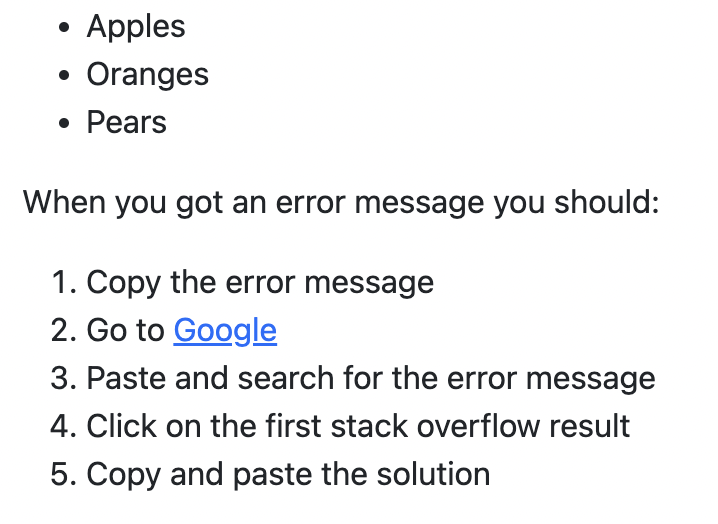
\includegraphics[width=10cm]{images/ch5-ulol.png}

\subsection*{Changing the default behaviour}

Remember that the first word in each line would be regarded as a tag. But you sometimes don't want that. 
\vspace{6mm}

For example, you might want to split the text of a \texttt{p} tag into multiple lines when the text is too long. You can actually put a \texttt{.} after the tag, and it now regards what indented within the tag as plain text, instead of regarding each first word of each line (e.g. \texttt{Hello}, \texttt{I}) as tags.

\begin{lstlisting}[language=pug]
p.
	Hello, I am KidProf.
	I am a university student studying Computer Science.
	I like coding.
\end{lstlisting}


\includegraphics[width=15cm]{images/ch5-textinaline.png}

\subsection*{\texttt{br} - using normal HTML syntax in Pug}
\label{sec:br}

But when you look at the output, they are all on the same line. This is because the line breaks you made in the code is independent of the line breaks shown on the web page, \textbf{you need to explicitly use \texttt{br} tags for line breaks}. Because we are inside the \texttt{p} tag, Pug regards everything inside as text but not tags, but we can still use conventional HTML syntax to get around it.

\begin{lstlisting}[language=pug]
p.
	Hello, I am KidProf. <br />
	I am a university student studying <br />Computer Science.<br />
	I like coding.
\end{lstlisting}


\includegraphics[width=15cm]{images/ch5-textmultiplelines.png}

Alternatively, if you do not like that normal HTML code in your Pug code, you could do this instead and lead to the same result. But this is a lot of effort and affects code readability.

\begin{lstlisting}[language=pug]
p
	| Hello, I am KidProf.
	br
	| I am a university student studying
	br
	| Computer Science.
	br
	| I like coding.
\end{lstlisting}

The removal of the \texttt{.} after \texttt{p} indicates that what indented within are tags instead of plain text, so the \texttt{br} tags are registered. To indicate that the rest are plain text, the \texttt{|} character is used.
\vspace{6mm}

\subsection*{Example}

Here is an example of an abouts page I did for a book reading project in middle school.

\begin{figure}[h]
\centering
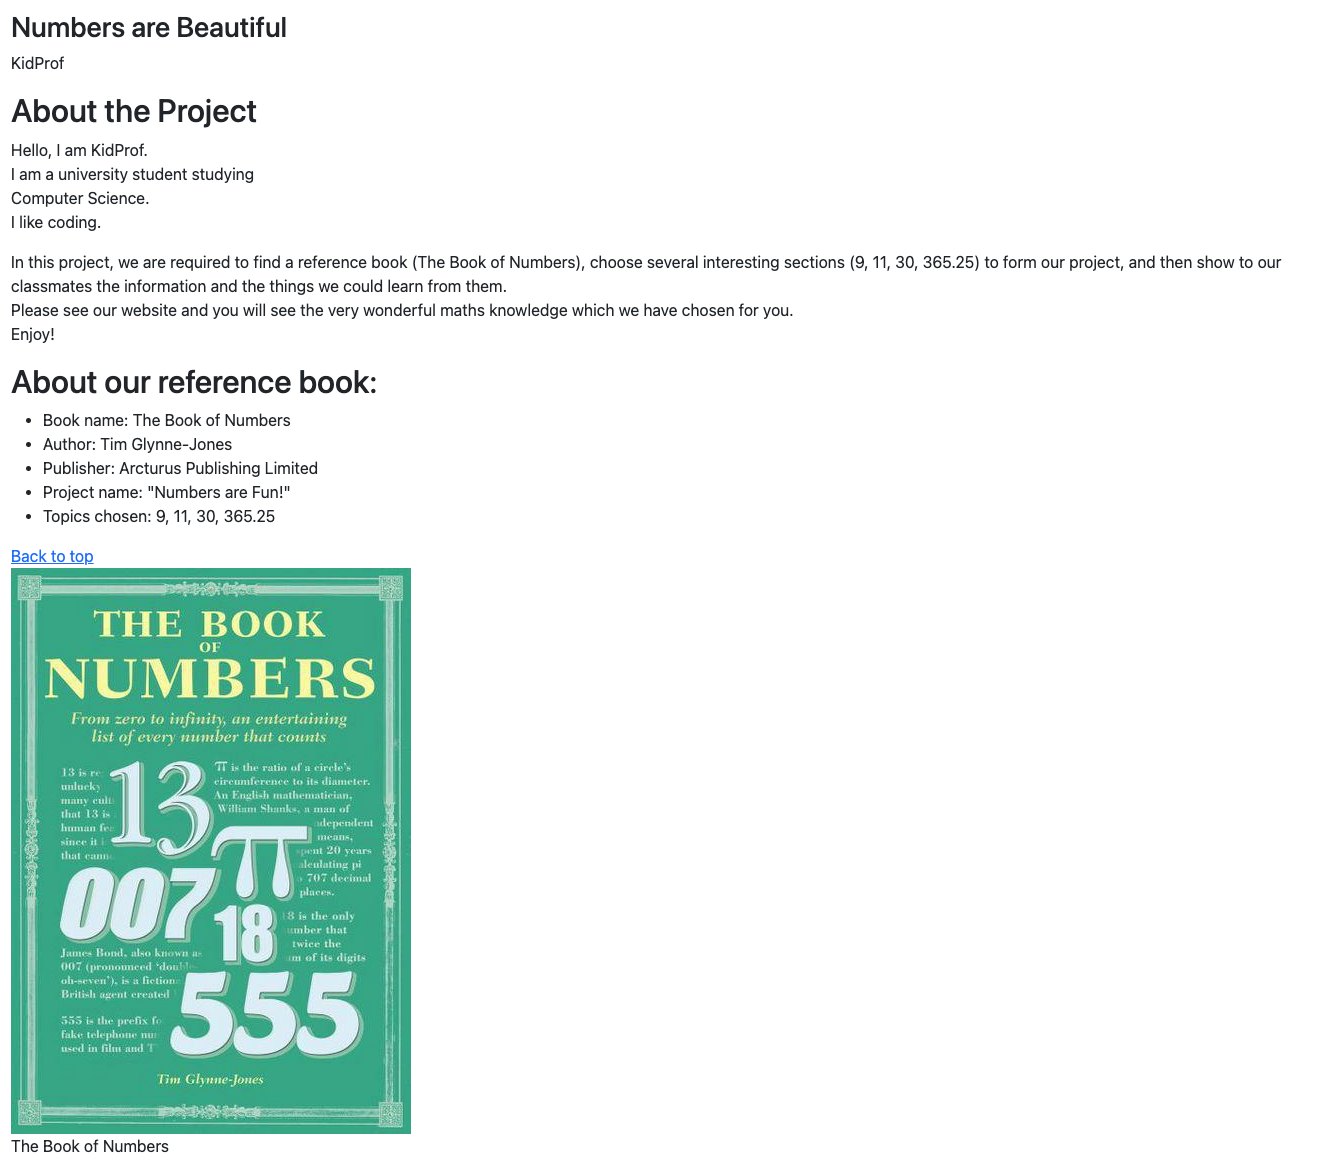
\includegraphics[width=15cm]{images/ch5-finalproduct.png}
\caption{Result of the code of the abouts page up till \cref{sec:list}}
\end{figure}

\begin{lstlisting}[language=pug]
//- templates/views/abouts.pug
h3 Numbers are Beautiful
p KidProf
h2 About the Project
p.
    In this project, we are required to find a reference book (The Book of Numbers), choose several interesting sections (9, 11, 30, 365.25) to form our project, and then show to our classmates the information and the things we could learn from them. <br />
    Please see our website and you will see the very wonderful maths knowledge which we have chosen for you. <br />
    Enjoy!
h2 About our reference book:
ul
    li.large-text Book name: The Book of Numbers
    li Author: Tim Glynne-Jones
    li Publisher: Arcturus Publishing Limited
    li.large-text Project name: "Numbers are Fun!"
    li.large-text Topics chosen: 9, 11, 30, 365.25
a(href="https://google.com") Back to top
br
img(src="images/bookofnumbers.jpg")
p The Book of Numbers
\end{lstlisting}

The behaviour of redirecting to Google when "Back to top" is clicked is not desirable and will be fixed in \cref{sec:vsclassesids}.

\section{Basic styling with classes and IDs}
\label{sec:classesids}

\subsection{Basic styling}

We need to introduce you to the basics of styling before we can really talk about classes and IDs.

We write our styles under \texttt{app/styles/site}, for now we can write all our styles in \texttt{layouts.less}. The styles we write are all in the following format. 

\begin{lstlisting}[language=pug]
//- app/styles/site/layouts.less
h2{
    color: red;
}
\end{lstlisting}

We need to tell the browser which elements we want to style, that is before the curly braces. Then, what's inside the curly braces are the styles that we want to apply to the concerned elements. Each style is followed by a semi-colon.
\vspace{6mm}

Those of you who have learnt CSS before may realise that it is exactly the same as CSS. This is true and this idea will be further explored later.
\vspace{6mm}

The easiest way is to reference the elements using tags, the style above applies to all \texttt{h2} tags in the whole web page. 

However, making all the \texttt{h2} tags red is not usually what we want. To style for specific elements, we would add a class or an ID to the element in the pug file, as an identifier of that particular element. then reference the class or ID in our less file.

\subsection{IDs}

We need the notion of classes and IDs to do styling in \cref{sec:styling}, so that we can reference elements that we would like to style from the styling files.

We use \texttt{\#} followed by text to indicate an ID, and we use \texttt{.} followed by text to indicate a class. ID and class names must not contain spaces, it is a convention to either use camelCase or hyphens in place of spaces.
\vspace{6mm}

For example, let's add an ID to the About the Project \texttt{h2} tag.

\begin{lstlisting}[language=pug]
//- templates/views/abouts.pug
...
    h2#red-header About the Project
... 
\end{lstlisting}

Then reference it in our less file instead of referencing all \texttt{h2} tags in the whole web page.

\begin{lstlisting}[language=pug]
//- app/styles/site/layouts.less
#red-header{
    color: red;
}
\end{lstlisting}

\subsection{Classes}

\textbf{IDs must be unique within a page, while there can be multiple elements with the same class name in the same page.} An element can have more than one class.
\vspace{6mm}

Now, let's define a new class named \texttt{large-text} to reference some \texttt{p} tags that we want to enlarge.

\begin{lstlisting}[language=pug]
//- templates/views/abouts.pug
ul
    li.large-text Book name: The Book of Numbers
    li Author: Tim Glynne-Jones
    li Publisher: Arcturus Publishing Limited
    li.large-text Project name: "Numbers are Fun!"
    li.large-text.blue-text Topics chosen: 9, 11, 30, 365.25
\end{lstlisting}

\begin{lstlisting}[language=pug]
//- app/styles/site/layouts.less
.large-text{
    font-size: 1.25rem;
}
\end{lstlisting}

We would explain the effect and syntax of different styles in detail in later sections. The difference between using IDs and classes would be explained in the \hyperref[sec:nestedstyles]{nested styles session}.

\subsection{div tags}

It serves no purposes in adding content to the web page, but it can be used to improve organisation of your code, and it is crucial for styling. 

For example, we are adding a \texttt{div} tag at the top with an id \texttt{\#quote}, surrounding the \texttt{h3} tag and the \texttt{p} tag.
\vspace{6mm}

\begin{lstlisting}[language=pug]
//- templates/views/abouts.pug
div#quote
    h3 Numbers are Beautiful
    p KidProf
h2#red-header About the Project
...
\end{lstlisting}
\vspace{6mm}

Then we can style that particular \texttt{h3} tag and \texttt{p} tag like this:
\vspace{6mm}

\begin{lstlisting}[language=pug]
//- app/styles/site/layouts.less
#quote h3{
    text-align: center;
    font-style: italic;
}
#quote p{
    text-align: right;
}
\end{lstlisting}
\vspace{6mm}

Spaces when specifying the elements for styling means "inside". For example, the first style will affect all \texttt{h3} tags (where there is only one) \textbf{inside} the \texttt{\#quote} div.

\subsection*{Some simplifications}
Because \texttt{div} tags are usually associated with classes and IDs, the keyword \texttt{div} can be omitted if you have at least one class or IDs associated with it. For example, \texttt{\#quote} is equivalent to \texttt{div\#quote}.
\vspace{6mm}

\begin{lstlisting}[language=pug]
//- templates/views/abouts.pug
#quote
    h3 Numbers are Beautiful
    p KidProf
h2#red-header About the Project
...
\end{lstlisting}
\vspace{6mm}

Also, we can write the styles for the quote ID like this alternatively. This is useful when there are many children inside a parent ID.
\vspace{6mm}

\begin{lstlisting}[language=pug]
//- app/styles/site/layouts.less
#quote {
    h3{
        text-align: center;
        font-style: italic;
    }
    p{
        text-align: right;
    }
}
\end{lstlisting}
\vspace{6mm}

\subsection*{Classes VS IDs}
\label{sec:vsclassesids}

IDs are more restrictive than classes. But we can do something more with IDs because only IDs can uniquely identify an element within the page.

To demonstrate one of the uses of IDs, we can modify the \texttt{href} attribute of the \texttt{a} tag. 

\begin{lstlisting}[language=pug]
//- templates/views/abouts.pug
...
a(href="#quote") Back to top
...
\end{lstlisting}

Now when you click on it, it brings you to the start of the page (if you zoom in large enough), to the element with ID \texttt{quote}, which is the top of the page. This feature does not work for classes because multiple elements can have the same class name in the same page.

\begin{figure}[h]
\centering
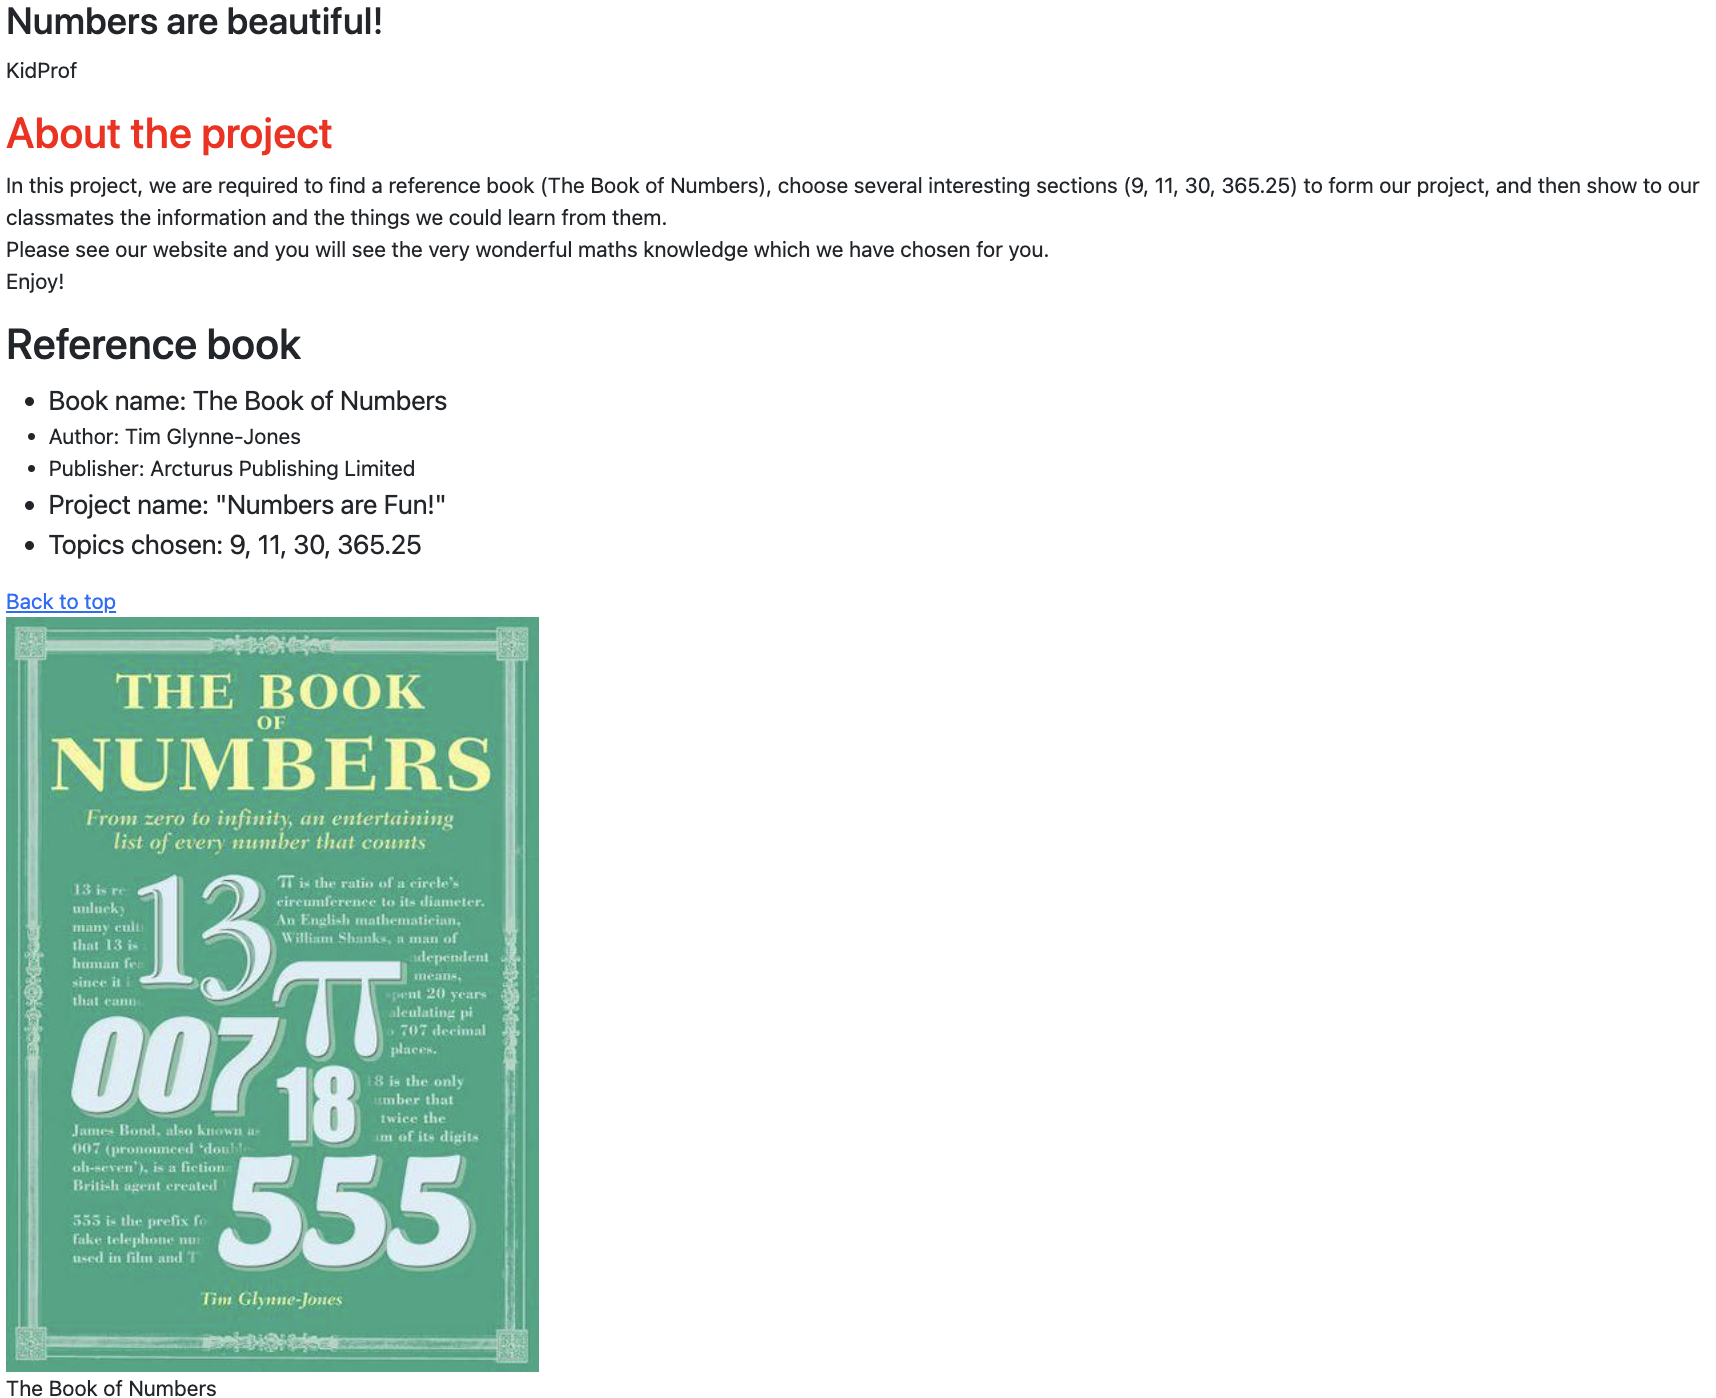
\includegraphics[width=15cm]{images/chn2-abouts-styled.png}
\caption{Result of the code of the abouts page up till \cref{sec:classesids}}
\label{fig:aboutspage}
\end{figure}

\newpage
\section{Summary: Pug VS HTML syntax}
\label{sec:pugvshtml}

\textit{This section aims to allow HTML programmers to relate what we are learning to what they have learnt. It is also a good chapter summary for those of you who have not learnt HTML before.}
\vspace{6mm}

\begin{itemize}
\item Pug uses indentation to indicate that something is in a tag while HTML uses closing tags. Each line corresponds to a single tag normally. On the other hand, indentation and next lines are not important in HTML syntax.
\vspace{6mm}

\begin{lstlisting}[language=pug]
//- pug
ul
  li A
  li B
  li C
\end{lstlisting}

\begin{lstlisting}[language=html]
<!-- HTML - poorly formatted, but would still work! -->
<ul><li>A</li><li>B</li><li>C</li></ul>
\end{lstlisting}

\item All attributes should be put within parenthesis after the tag in Pug, while attributes should be put within the opening tag in HTML.
\vspace{6mm}

\begin{lstlisting}[language=pug]
//- pug
a(href="abouts.html") Click to go to the abouts page.
\end{lstlisting}

\begin{lstlisting}[language=html]
<!-- HTML -->
<a href="abouts.html">Click to go to the abouts page.</a>
\end{lstlisting}

\item Classes and IDs declarations can be simplified with Pug using the syntax shown in \cref{sec:classesids}. The \texttt{div} keyword can also be omitted when used with classes and IDs.
\vspace{6mm}

\begin{lstlisting}[language=pug]
//- pug
a#abouts-link.class1.class2(href="abouts.html") Click to go to the abouts page.
\end{lstlisting}

\begin{lstlisting}[language=html]
<!-- HTML -->
<a href="abouts.html" id="abouts-link" class="class1 class2">Click to go to the abouts page.</a>
\end{lstlisting}

\end{itemize}
